% First Draft for ECON807 Policy Project
% Daniel Sánchez Pazmiño
% ECON807 Spring 2023

% Requires the data-preparation.R to run.

\documentclass[11pt,a4paper]{article}\usepackage[]{graphicx}\usepackage[]{xcolor}
% maxwidth is the original width if it is less than linewidth
% otherwise use linewidth (to make sure the graphics do not exceed the margin)
\makeatletter
\def\maxwidth{ %
  \ifdim\Gin@nat@width>\linewidth
    \linewidth
  \else
    \Gin@nat@width
  \fi
}
\makeatother

\definecolor{fgcolor}{rgb}{0.345, 0.345, 0.345}
\newcommand{\hlnum}[1]{\textcolor[rgb]{0.686,0.059,0.569}{#1}}%
\newcommand{\hlstr}[1]{\textcolor[rgb]{0.192,0.494,0.8}{#1}}%
\newcommand{\hlcom}[1]{\textcolor[rgb]{0.678,0.584,0.686}{\textit{#1}}}%
\newcommand{\hlopt}[1]{\textcolor[rgb]{0,0,0}{#1}}%
\newcommand{\hlstd}[1]{\textcolor[rgb]{0.345,0.345,0.345}{#1}}%
\newcommand{\hlkwa}[1]{\textcolor[rgb]{0.161,0.373,0.58}{\textbf{#1}}}%
\newcommand{\hlkwb}[1]{\textcolor[rgb]{0.69,0.353,0.396}{#1}}%
\newcommand{\hlkwc}[1]{\textcolor[rgb]{0.333,0.667,0.333}{#1}}%
\newcommand{\hlkwd}[1]{\textcolor[rgb]{0.737,0.353,0.396}{\textbf{#1}}}%
\let\hlipl\hlkwb

\usepackage{framed}
\makeatletter
\newenvironment{kframe}{%
 \def\at@end@of@kframe{}%
 \ifinner\ifhmode%
  \def\at@end@of@kframe{\end{minipage}}%
  \begin{minipage}{\columnwidth}%
 \fi\fi%
 \def\FrameCommand##1{\hskip\@totalleftmargin \hskip-\fboxsep
 \colorbox{shadecolor}{##1}\hskip-\fboxsep
     % There is no \\@totalrightmargin, so:
     \hskip-\linewidth \hskip-\@totalleftmargin \hskip\columnwidth}%
 \MakeFramed {\advance\hsize-\width
   \@totalleftmargin\z@ \linewidth\hsize
   \@setminipage}}%
 {\par\unskip\endMakeFramed%
 \at@end@of@kframe}
\makeatother

\definecolor{shadecolor}{rgb}{.97, .97, .97}
\definecolor{messagecolor}{rgb}{0, 0, 0}
\definecolor{warningcolor}{rgb}{1, 0, 1}
\definecolor{errorcolor}{rgb}{1, 0, 0}
\newenvironment{knitrout}{}{} % an empty environment to be redefined in TeX

\usepackage{alltt}

% ========================================= Preamble ========================================= %

% ---- Document Parameters ---- %

\title{The influence of entry regulation on formal employment \\[1em] 
\large{ECON 807 Macroeconomic Theory \& Policy Policy Project Draft}}
\author{Daniel Sánchez Pazmiño}
\date{March 2023}

% ---- Load LaTeX packages ---- %

% Format

\usepackage[margin = 1in]{geometry}

% Referencing

\usepackage[backend = biber, style = apa, citestyle = apa]{biblatex}
  \addbibresource{refs.bib}

% Misc

\usepackage{lipsum}

% ---- Preamble Chunks ----- %



% ----- Document ----- % 
\IfFileExists{upquote.sty}{\usepackage{upquote}}{}
\begin{document}

\maketitle

\begin{abstract}

\lipsum[1]

\end{abstract}

\section{Introduction}

It is well known that informal work -legal but informal economic activities which occur outside the government's regulatory capability \parencite{Sassen.1994} - can hinder economic development through several channels. Informal firms reduce the amount of taxes that can be collected by governments and these businesses tend to remain small and inefficient. Additionally, workers in the informal sector usually lack access to social security and other employment benefits and tend to earn lower wages even after controlling for skills. Informality is also related to bigger gender gaps, higher inequality, lower education and several other factors which worsen economic outcomes \parencite{Delechat2020}. Further, the informal economy has been characterized with poorly defined work spaces, unsafe and unsanitary working conditions, inconsistent pay, long working hours and a lack of access to markets, financial services, training, and technology \parencite{IloND}. 

While less present in the developed world, informality seems to be very prevalent in developing countries, where it represents a third of low and middle-income countries' economic activity \parencite{Delechat2020}. In the world, the informal economy is thought to encompass more than half of the labour force and more than 90\% of small and micro businesses. The work of \textcite{Soto.2002} has motivated much research about informality in Latin America, being one of the regions with the most prevalent levels of informality, as it often is the only option for several workers on the lower end of the wealth distribution \parencite{Oviedo.2009}. At the macroeconomic level, informality could be regarded as one consequence of poor institutions, which have been shown to be significant factors for growth \parencite{Acemoglu.2001, RafaelLaPorta.1997, Glaeser.2004}. Further, its effect on inequality and its potential to be a channel for the propagation of monetary and fiscal policy \textcite{Alberola.2020} make informality a significative macroeconomic determinant of underdevelopment.

The desire for the formalization of the economy is well understood, especially considering that the impact on economic activity due to COVID-19 has increased informality worldwide \parencite{ILO.2022}. However, the policy angle to this issue is subtle, given that the causes and consequences of informality are difficult to document and understand. Among others, some policy approaches have focused on the role of governments in providing incentives for formalization. One approach has been to design tax systems that minimize distortions in the market \parencite{Bardey.2019} as well as reducing the costs of formalization by reducing entry regulation for firms. As proposed by \textcite{MauricioPrado.2011}, firms which are less productive endogenously choose to operate in the informal sector due to entry costs and taxation in the formal sector. While larger firms might be able to overcome the costs of formalization, smaller, less productive firms may not; thus, reducing entry costs can directly affect entrepreneurship.

\begin{figure}[h]
\caption{Active formal businesses and job contracts registered under Social Security in Ecuador (2018-2022)}
\begin{knitrout}
\definecolor{shadecolor}{rgb}{0.969, 0.969, 0.969}\color{fgcolor}
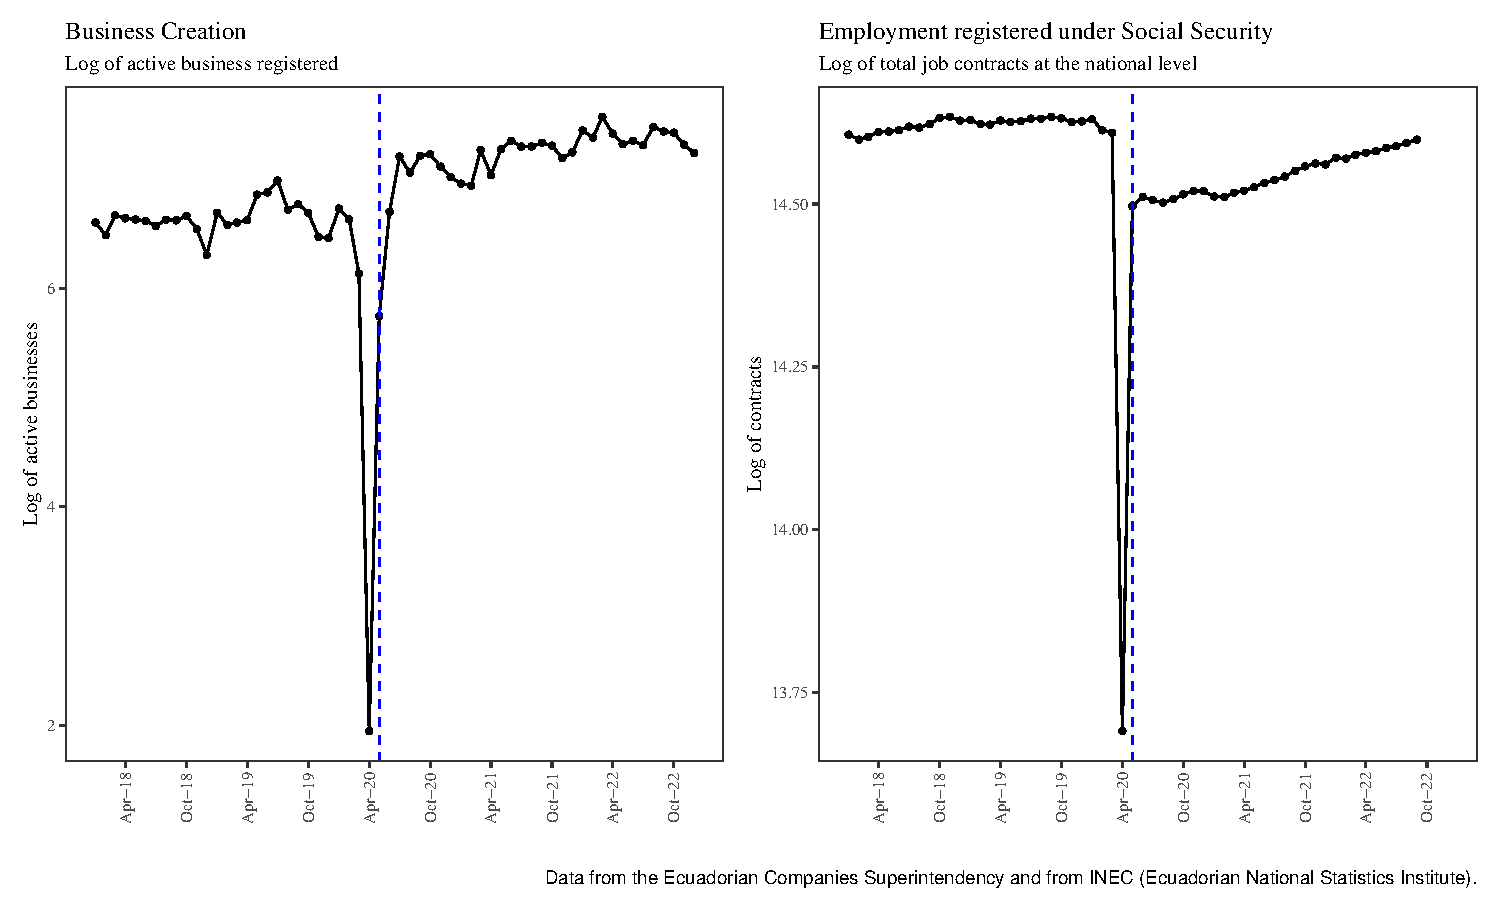
\includegraphics[width=\maxwidth]{figure/figure-1-1} 
\end{knitrout}
\end{figure}

In this paper, I investigate the relationship between entry regulation and labour market formalization by exploiting an exogenous shock on entry regulation in post-pandemic Ecuador. By using administrative data of various Ecuadorian public institutions, Through a comprehensive event study empirical framework, I exploit variation across time at the province level in Ecuador before and after the reform. The policy change was enacted in May 2020 and allowed for the creation of a new legal form of business, the \textit{Sociedad de Acciones Simplificada}\footnote{\textit{Simplified Shares Society.}} (SAS). The reform sought to impact reduced monetary and time costs relative to other legal figures in the firm creation process, and has proven to be effective in doing so \textcite{CaminoMogro.2022}. Although business creation can be intuitively related to job creation in the formal sector, and such correlation is vivid in Ecuadorian data (see Figure), no other paper has studied the labour market effects of this reform.

I base the empirical analysis under a theoretical framework informed by the work of \textcite{Branstetter.2014}. In a simple model of entrepreneurship, it is predicted that reduced entry costs will positively impact firm entry and employment, however, all increases are at the margin: while new firms will enter the (formal) sector, these firms will be generally smaller, less productive and less likely to hire large amounts of new workers. The results from the empirical analysis initially show a positive significative effect of the reform on employment, however, the effect is not robust to different specifications. Further, event study specifications suggest that due to the timing of the policy, the immediate effects of the policy might be due to catchup effects from the pandemic rather than due to the underlying economic mechanism of the reform. These results suggest that the true causal effect of the policy on employment is too small to identify with my empirical strategy or even null. The empirical validations of the entrepreneurship model \textcite{Branstetter.2014} in Portugal \parencite{Branstetter.2014} and Mexico \parencite{Kaplan.2011} find small positive effects of entry cost deregulation, however, the posiblity of a null effect of the reform in Ecuador might be explained by the lack of coordination between entry and labour market regulation. 

Through this paper, I contribute to the very reduced stream of research which analyses the impact of entry regulations on employment, considering the existence of informal and formal sectors. Further, the use of administrative instead of survey data enhances the possibilities of extracting insight which is valid at any level of disaggregation and also enhance data quality of the reporting of formal employment. To my knowledge there has been no research which links these type of policies to the creation of formal employment, given that these policies are geared towards fostering entrepreneurship and often labour markets are tackled through other types of policies. However, given that \textcite{Branstetter.2014} identifies marginal firms as smaller, which are more likely to be informal \parencite{ElianeElBadaoui.2010}, entry cost regulation may be an important policy tool for tackling informality, specially when labour market reform is politically blocked, as is the case of Ecuador. 

\section{Literature Review}

The literature on informality and entry cost regulation is extensive. The theoretical framework points to informality being an endogenous decision, where firms with low productivity often prefer to remain informal, the size of the firm often being an important determinant of this decision \parencite{Delechat2020, MauricioPrado.2011, ElianeElBadaoui.2010}. The fact that informality is an endogenous decision makes informality difficult to investigate empirically; many informal workers are not officially registered and may not report their activities accurately \textcite{Oviedo.2009}. 

Apart from the consensus finding that informality reduces growth and developmental outcomes, in the macroeconomic context, it has been shown that informality lowers TFP and increases output volatility and may produce significant input misallocation. Further, informal jobs have been found to respond heavily to changes in formal employment \parencite{Leyva.2020}. This allows me to use formal jobs data, which is easier to obtain and is usually not sensitive to its definition, as are informal jobs. Further, \textcite{Lambert.2020} proposes that informality plays a shock-absorbing role due that it limits movements in the employed-unemployed margin. This is very relevant to the Ecuadorian case, as the country often shows a relatively low rate of unemployment which is deemed to be uninformative due to the prevalence of underemployment \parencite{LaTorre.2017}.

Research on Ecuadorian informality is limited and has often focused on the effect of exogenous shocks on measurements of informality, notably measuring the effects of a significant earthquake in 2016 \parencite{Mendoza.2020} and the labour market impact of Venezuelan migration \parencite{Olivieri.2022}, both finding positive effects on informality. It is determined that poverty and informality are jointly determined, where informal workers often come from low-education and income backgrounds. Further, the informal labour market is mainly supply-led but it is so heterogenously: low-skilled workers often have no choice to work informally, while better educated workers sometimes choose to operate informally \parencite{Canelas.2019}. The minimum wage seems to produce no clear effect on informality due to high non-compliance \parencite{Canelas.2014}. A firm size wage premium has been shown to appear across developing countries, which \textcite{ElianeElBadaoui.2010} proposes that responds to informality. Ecuador has proven this theoretical prediction of formal firms often paying more to their employees due to them being larger \textcite{MacIsaac.1997}. On the firm side, it is determined that the endogenous choice of sector is also present in Ecuador \textcite{Medvedev.2016}. 

Estimating the size and nature of the informal economy and to assess the impact of policies aimed at reducing informality is difficult, however, one common idea that has come up as a policy angle is reducing distortions for businesses by simplifying entry regulation to facilitate formal entry for businesses. These type of policies have been implemented widely across Latin America as well as in Europe, which have had positive results \parencite{Oviedo.2009}. 

However, the research has been focused on these policies effectiveness at creating formal businesses, not on measuring their labour market impact. \textcite{Branstetter.2014} develop a simple entrepreneurship model and validate it with a reduction of entry costs in Portugal, finding the reform significantly impacted business creation but mostly for marginal firms. These marginal firms were typically small, owned by relatively poorly educated entrepreneurs, and operating in low-technology sectors and were less likely to survive their first two years. Employment effects of the reform were positive but small, as was the case of a Mexican deregulation of entry by \textcite{Kaplan.2011}. Further, \textcite{Bertrand.2002} find that both product market and entry regulation were sources of employment growth in France in the 1970s, focusing on the retail sector in France. Further, a macroeconomic study of product and labour market regulation, modelled as higher entry costs, links higher levels of regulations to lower employment \parencite{Blanchard.2003}. 

\section{Theoretical Framework}

I utilize the theoretical model of entrepreneurship proposed by \textcite{Branstetter.2014} to guide my empirical analysis. In this model, the economy is comprised of individuals with different entrepreneurial ability endowments $\theta$, drawn from a continuous probability distribution and the possibility to (a) work in the labour market for a wage rate $w$, (b) become an entrepreneur or (c) consume leisure. The payoff to being an entrepreneur, $\pi$ is

\begin{equation}
  h(\theta) + \eta
\end{equation}

where $h$ is a function of the agent's entrepreneurial ability and $\eta$ is an idiosyncratic term, also distributed across the economy from a probability distribution and unknown to the entrepreneur before starting their business operation. By defining $h$ as Cobb-Douglas, considering only labour $L$ as a production input and introducing two periods, it is possible to define two profit functions, where the difference between the two is that a fixed cost $F$ is included in $\pi_t$ for $t = 1$ but not for $t=2$ and that the stochastic term $\eta$ is revealed to the agent in $t=2$. The value for operation as an entrepreneur depends on the level of entrepreneurial ability relative to the prevailing market wage rate $w$, as well as the fixed cost $F$. The model predicts that a decrease on entry costs translates to a reduction of fixed cost $F$ and thus increases the value of entrepreneurship, allowing for a larger number of agents entering the economy as businesses. 

Further, the level of employment in this economy depends on the level of entrepreneurship, and each entrepreneur's labour demand will depend once again on their endowment $\theta$ relative to the market wage $w$. Any decrease in $F$ will increase the level of employment, considering that there will be more entrepreneurs in the economy. However, since reductions in $F$ will work \textit{at the margin}, all extra entrepreneurs generated by the policy change will have relatively low $\theta$ and thus smaller labour demand.

This model does not consider the level of capital $K$ and liquidity constraints, and assumes that all workers are hired formally. By observing formal employment fluctutations, it is possible to apply this model to the empirical analysis. However, the model is not able to explain changes in informal employment per se, only changes in formal employment. The extent to which changes in formal employment relate to informal employment is dependent on the ability to observe the pre-policy status of workers hired after the policy change.

\section{Institutional Background}

Ecuador is a middle income country located in upper South America next to Colombia and Peru. After its full dollarization in 2000, the country saw an economic surge between 2007-2014 as a result of high oil prices and a relatively indebted government \parencite{Weisbrot.2017}. However, after a sharp decline in oil prices and the COVID-19 pandemic, the country seems to be unable to return to its pre-pandemic or pre-2014 levels, with employment indicators at an all-time low. 

However, informality and underemployment in this labour market have been shown to be historically high \parencite{Meneses.2021, Chavez.2012, Mendoza.2020}. It has been determined that minimum wage increases in Ecuador (which have been frequent and substantial) have had virtually no effect on employment levels due to high-level of non-compliance and informality in the labour market \parencite{Canelas.2014}. Further, Ecuador has been shown to have one of the most cumbersome labour market legislations in the region \parencite{MacIsaac.1997}, whose effect is attenuated by smaller base earnings over which benefits are paid, which suggests a correlation between lower wages and higher amount of labour market regulation. 

Not only the labour market is highly regulated in the country: the business environment in Ecuador is cumbersome, including several artificial costs which could create inefficiencies. Ecuador constantly ranks very low in terms of property rights, judicial transparency and economic freedom. Its low standing in economic freedom responds to a flawed and corrupt judiciary, characterized by inefficiency and difficulty to start a business \textcite{Euromonitor.2022}. Further, an unstable economic and political environment after the election of conservative businessman Guillermo Lasso not long after a decade-long leftist regime has taken a toll on the government's financing capabilities. 

The political instability has also made the deregulation of labour markets difficult only one set of market-friendly policies set forth by the new president have been passed, the labour market reform being immediately rejected by a strong opposing majority in Congress. Thus, other types of reforms which indirectly target the labour market would be welcome. 

The SAS reform, enacted in May 2020, allowed a new type of legal business to exist, which also exists in other countries in the region. This type of business is known to be much less burdensome than other types of companies like anonymous societies or limited liability companies. A SAS business can be created with lower monetary and time costs (notarization, registering, etc.) as well as with lower amounts of capital contributions. It is sensible to believe that the reform was unexpected and exogeneous since, while the law that allowed for this reform came into force in early 2020, the law did not specifically plan for the creation of this type of business, only allowed for its creation under the Ecuadorian corporate law. Further, \textcite{CaminoMogro.2022} find causal evidence that this reform was effective in formalizing/creating businesses and in reducing time and money entry costs. However, the effects of the policy in the labour market have not been studied so far. 

\section{Methodology}

\subsection{Data}

\subsection{Empirical Strategy}

\section{Results}

\end{document}
